%# -*- coding: utf-8-unix -*-
% !TEX program = xelatex
% !TEX root = ../thesis.tex
% !TEX encoding = UTF-8 Unicode
%%==================================================
%% chapter02.tex for SJTU Master Thesis
%% based on CASthesis
%% modified by wei.jianwen@gmail.com
%% Encoding: UTF-8
%%==================================================


\chapter{Competition on two layer with different structural network}
\label{chap:competition on two layer with different structural network}
In this chapter, based on the competition model described in previous chapter, simulation would be implemented with changing the network structures. Network structures would be altered by changing the internal and external edges with random regular network and Barabasi-Albert network. 

\section{Competition on Random Regular Networks}
In this section, each layer consists of random regular network that has $N$ nodes with $k$ internal edges as introduced in \cite{kimsangwoo2012, bela2001}. Each node of one layer is connected with a random node on the other layer. This means each node has only $1$ external un-directed edge. Simulations are preformed on network with $N=2048$, and $k = 5$. 

The simulation results are shown in Fig.~\ref{Fig2} and Fig.~\ref{Fig3}. Fig.~\ref{Fig2}(a) shows that when $\gamma > 0.4$, $1.2 < \beta < 1.95$, it normally tends to positive consensus. But, if $\beta$ is lower or larger than certain values, it doesn't make consensus.
In Fig.~\ref{Fig2}(b), as $\beta$ increases, it normally change from positive to negative consensus. But, when $\gamma$ is very low($\gamma \le 0.1$), it doesn't make positive consensus. On the other hand, when $\gamma$ is large enough, it makes positive consensus. But, when $\beta$ is large enough, it is changed into negative consensus. When both of $\gamma$ and $\beta$ are large enough, the state is in a coexistence part.

\begin{figure*}[!htb]
	\centering
	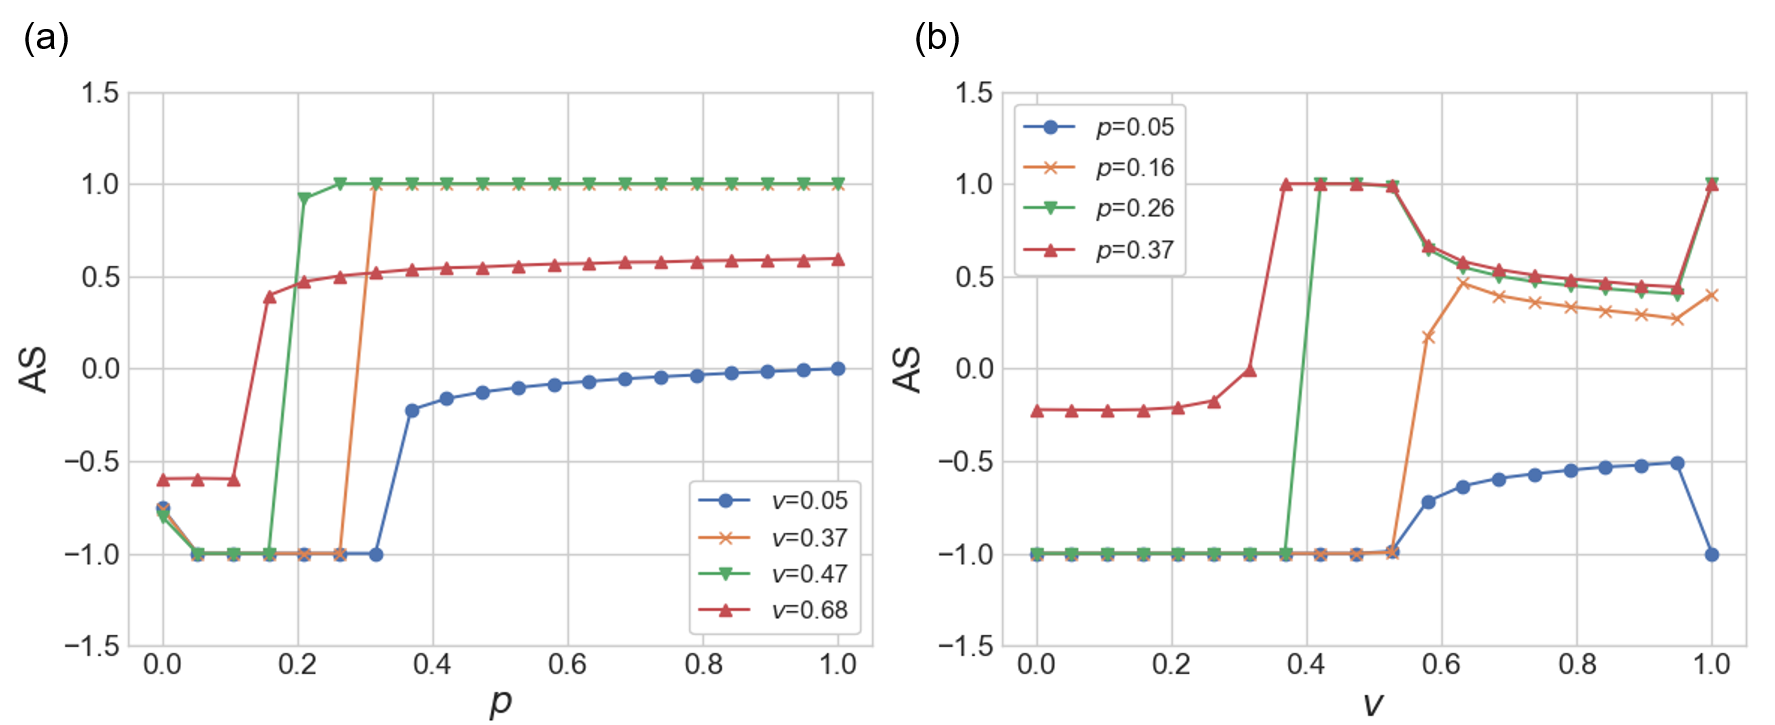
\includegraphics[width=\hsize]{AS_2d.png}
	\caption{(a) $p$-\textit{AS} chart according to certain $v$ values. (b) $v$-\textit{AS} chart according to certain $p$ values.}
	\label{AS_2d}
\end{figure*}

\begin{figure}[!htb]
	\centering
	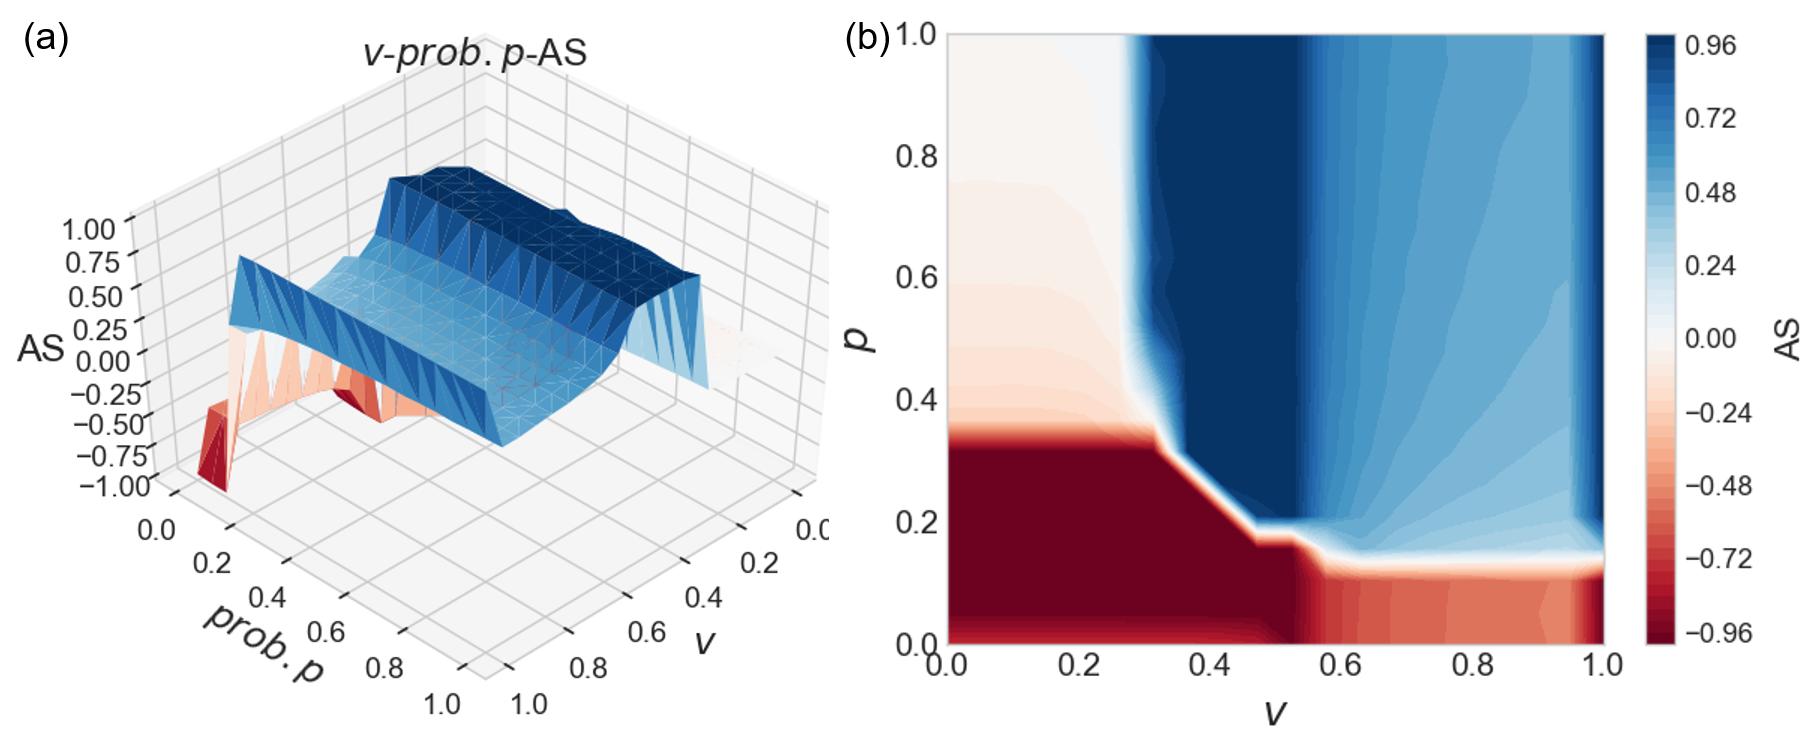
\includegraphics[width=\hsize]{p_v_AS_3d.png}
	\caption{Two layer networks with sequential updating rule : \textit{AS} changing with all $p$ and $v$}
	\label{p_v_AS_3d}
\end{figure}


\begin{figure}[!htb]
	\centering
	\includegraphics[width=\hsize]{FIG3.png}
	\caption{Random Regular Networks : \textit{AS} changing with $\gamma$ and $\beta$}
	\label{Fig3}
\end{figure}

Fig.~\ref{Fig3} shows the states of two layers according to all $\gamma$s and all $\beta$s. The $X$-axis is the $\gamma$ and the $Y$-axis is the $\beta$, and the $Z$-axis represents \textit{AS}. The closer the color is to blue, the more it has positive consensus. And the closer the color is to red, the more it has negative consensus. A light and white areas have coexistence with positive states and negative states. This chart has two areas for coexistence, when $\beta$ is very low or very high. When $\beta$ is in certain range, interconnected network can perform positive or negative consensus with different $\gamma$ values

\section{Competition on Networks with different number of external links}

In this section, we consider the influence of external links. Based on the basic model in Subsection 3.1, we reduce the number of nodes in layer B at a certain rate and increase the external links from nodes in layer B accordingly.  We denote \textit{HM(n)} as a hierarchical model with a level $n$, which means that the number of nodes in layer B is $1/n$ of the number of nodes in layer A, and the number of external links from node in layer B is $n$ in view that the number of external links from node in layer A is $1$. In other words, each node in layer A has one external edge, but each node in layer B has $n$ external edges for \textit{HM(n)}, which means one node in layer B can be influenced by $n$ nodes in layer A. $\gamma$ scale is same as the Random Regular Networks Model. But, $\beta$ scale depends on the number of degrees. So the $\beta$ scale is adjusted to have the same probability of volatility with Random Regular Networks Model(\textit{RRM}) as following Equation.
\begin{equation}
{\beta _{h,\max}} = {\beta _{rr,\max}} \cdot \log \left( {\frac{{{n_{rr}}^{ - {S_i}}}}{{{i_{rr,i}} + {e_{rr,i}}}} \cdot \frac{{{i_{h,i}} + {e_{h,i}}}}{{{n_{h}}^{ - {S_i}}}}} \right). 
\end{equation}

Eq(6) is derived from Eq(1) at the initial states. $\beta _{h,\max}$ is the maximum value of $\beta$ scale in \textit{HM}, and $\beta _{rr,\max}$ is the maximum value of $\beta$ scale in \textit{RRM}. When \textit{RRM} begins with initial state and the maximum of $\beta$ scale, it has the lowest volatility except $0$. In order to have the same probability in layer B dynamics for different network structures at the initial time, maximum value of $\beta$ in \textit{HM} is calculated based on Eq(6). 

Fig.~\ref{Fig4} shows the Hierarchical Model simulation results. Comparing \textit{HMs} with \textit{RRM}, \textit{CR} and \textit{PCR} are all increased remarkably. \textit{HMs} have more positive consensus part than \textit{RRM}. It shows that as the number of B nodes are decreased, it is easy to make positive consensus. Comparing \textit{HM(16)} with other \textit{HMs}, \textit{HM(16)} has the most positive consensus part. In case of models where the number of nodes in layer B is less than \textit{HM(16)},  \textit{CR} and \textit{PCR} of the models are decreased and \textit{NCR} is increased slightly. Also, for models where the number of nodes in layer B is more than \textit{HM(16)}, \textit{CR} and \textit{PCR} are also decreased. However, \textit{HM(4)} has the most \textit{AS total}. Although \textit{HM(4)} doesn't have the most consensus part, it has more intensity for positive social opinion. It can be analyzed that strong social intensity usually can not make more consensus. These results indicate that network structure can contribute more for consensus. 

\begin{figure}[!htb]
	\centering
	\includegraphics[width=\hsize]{FIG4.png}
	\caption{Hierarchical Model(\textit{HM(n)})}
	\label{Fig4}
\end{figure}

In summary, all the Hierarchical Models have more consensus ratio than Random Regular Networks Model. Among \textit{HMs}, \textit{HM(16)} has the most positive consensus part. When the number of nodes in layer B is more or less than \textit{HM(16)}, \textit{CR} and \textit{PCR} are decreased. This shows that there exists an efficient number for the decision making layer to perform positive consensus.  

\section{Competition on Networks with different number of internal links}
\begin{figure}[!htb]
	\centering
	\includegraphics[width=\hsize]{figure/FIG5.png}
	\caption{Comparison of Networks with different internal degrees(\textit{RR(n)-RR(m)}: layer A has random regular network with $n$ internal edges, layer B has random regular network with $m$ internal edges)}
	\label{Fig5}
\end{figure}
Next, the interconnected networks are simulated with different internal degrees in order to define and evaluate the influence of internal degrees. The number of internal degrees on each node is switched to $2$ or $5$.

Fig.~\ref{Fig5} shows the simulation results with changing the number of internal edges. \textit{RR(5)-RR(2)} has the most \textit{PCR}. \textit{RR(2)-RR(5)} has the most \textit{NCR}. When the number of internal edges in layer A are more than layer B, it has more positive consensus. On the other hand, when the number of internal edges in layer B are more than layer A, it has relatively more negative consensus. These results provide that the number of edges on layer A has the tendency to keep positive state, and the number of edges on layer B has the tendency to keep negative state. The number of internal edges have the influence on consensus result and a layer with more internal edges has the tendency to maintain its own state. In case of networks with same internal edges, \textit{RR(2)-RR(2)} has more \textit{PCR} and \textit{AS total} than \textit{RR(5)-RR(5)}. It can be analyzed that \textit{RR(5)-RR(5)} is hard to make consensus, because it has more internal edges to cause inner conflict. Also, \textit{RR(2)-RR(2)} has less \textit{NCR} than \textit{RR(5)-RR(5)}. It shows that the number of internal edges in layer B is more sensitive than layer A. As Eq(1) shows, layer B dynamics can have more various and extreme probabilities when it has more degrees. For example, in case of \textit{RR(2)-RR(2)} with $\beta = 1$, the dynamics starts with $P_B=1/3$ and in case of \textit{RR(5)-RR(5)} with $\beta = 1$, the dynamics starts with $P_B=1/6$.    

\section{Competition on Networks with different structures}
So far, each layer of the interconnected network consisted of random regular networks that has the same number of edges for each node. Now, the simulation would be implemented on different network structures. 

\begin{figure}[!htb]
	\centering
	\includegraphics[width=\hsize]{FIG6.png}
	\caption{Comparison of Networks with different structures}
	\label{Fig6}
\end{figure}

Here, we use \textit{Barabasi-Albert network(BA)} structure as introduced in \cite{barabasi1999}. To evaluate the influence of network structure, 5 simulations are implemented with changing network structures. The \textit{BA} network is applied for both layers or switched on each layer. And, because layer A with \textit{BA} network structure has total $10,215$ internal edges, \textit{RR(10)-RR(5)}, under the similar conditions such as the number of nodes and edges, is also simulated. The simulation results are shown in Fig.~\ref{Fig6}. The result of \textit{BA-RR} and \textit{RR(10)-RR(5)} have almost the same features. The gap of \textit{CR} is almost same(less than 0.01). The structure of network make no obvious difference of consensus results. In case of \textit{BA-BA}, the \textit{CR} has the least ratio for consensus. \textit{BA-BA} structure has lots of internal edges on each layer. Therefore, it is hard to make consensus due to inner conflict on each layer. 

